\section{Experiments}

We organize our experiments around three questions. First, does \method{} improve upon vanilla OPD under the same long-context training and evaluation setup? Second, does residualizing group-normalized verifier feedback improve upon adding that feedback directly? Third, does relative-advantage-based credit assignment (RACA) improve upon uniform residual allocation?

\subsection{Experimental Setup}

\paragraph{Models.}

We use Qwen3-4B\footnote{\url{https://huggingface.co/Qwen/Qwen3-4B}} and Qwen3-8B\footnote{\url{https://huggingface.co/Qwen/Qwen3-8B}} as student models and Qwen3-30B-A3B-Thinking-2507\footnote{\url{https://huggingface.co/Qwen/Qwen3-30B-A3B-Thinking-2507}} as the teacher model. Both students operate in no-thinking mode. The teacher provides token-level log probabilities for OPD training.

\paragraph{Training data.}

We construct the training set from GoLongRL~\citep{lv2026golongrl} by retaining prompts no longer than 32K tokens. The resulting subset contains 9{,}527 prompts across nine task families. Table~\ref{tab:training-rewards} summarizes their distribution and native verifier metrics. Three task families use binary rewards, while the remaining six use graded rewards. The two largest families, precise long-range retrieval and evidence-grounded reasoning, account for 82.9\% of the training set.

\begin{table}[ht]
\captionsetup{justification=raggedright,singlelinecheck=false,skip=6pt}
\caption{Composition and reward interfaces of the 9{,}527-prompt GoLongRL subset after the 32K filter. ``B'' denotes a binary reward in $\{0,1\}$; ``G'' denotes a graded score in $[0,1]$.}
\label{tab:training-rewards}
\centering
\small
\setlength{\tabcolsep}{3.2pt}
\renewcommand{\arraystretch}{1.05}
\begin{tabular}{@{}l c l@{}}
\toprule
\textbf{Task Family} & \textbf{\# Samples} & \textbf{Native Verifier} \\
\midrule
Precise Long-Range Retrieval & 4,693 & Exact Match (B) \\
Evidence-Grounded Reasoning & 3,204 & Accuracy (B) \\
Multi-Table Extraction & 729 & IoU (G) \\
High-Recall Retrieval & 540 & Set F1 (G) \\
Fragment Matching and Induction & 148 & Subset EM (G) \\
Sequence Reconstruction & 69 & Pairwise Acc. (G) \\
Numerical Reasoning & 54 & Math Verify (B) \\
Graded Retrieval and Ranking & 45 & NDCG (G) \\
Long-Document Summarization & 45 & ROUGE-L (G) \\
\bottomrule
\end{tabular}
\end{table}


\ifdefined\GCOPDSingleColumnLayout\else
\ifdefined\GCOPDSingleColumnLayout
\begin{table}[t]
\else
\begin{table*}[t]
\fi
\caption{Qwen3-4B and Qwen3-8B results on five long-context benchmarks (\%). ``Avg.'' is the unweighted five-task mean. $\dagger$ denotes an implementation of the method's principal training-signal mechanism under the shared setup.}
\label{tab:main-results}
\centering
\small
\setlength{\tabcolsep}{4.0pt}
\begin{tabular}{l l c c c c c c }
\toprule
\multirow{2}{*}{\bf Model} & \multirow{2}{*}{\bf Method} & \multicolumn{6}{c}{\bf Benchmark} \\
\cmidrule(lr){3-8}
& & \bf Avg. & \bf DocMath & \bf Frames & \bf MRCR & \bf CorpusQA & \bf LBv1QA \\
\cmidrule(lr){1-2} \cmidrule(lr){3-8}
\multirow{7}{*}{Qwen3-4B}
& Raw & 29.08 & 43.63 & 26.58 & 22.02 & 6.99 & 46.20 \\
& OPD & 39.31 & 49.37 & \underline{30.95} & 26.90 & 32.22 & \textbf{57.10} \\
& ExOPD$^{\dagger}$ & 38.22 & 47.75 & 29.61 & 25.95 & 31.91 & 55.90 \\
& Uni-OPD$^{\dagger}$ & 38.53 & \textbf{51.88} & 29.98 & 27.93 & 27.36 & 55.50 \\
& PowerOPD$^{\dagger}$ & 38.88 & 49.63 & 30.10 & \textbf{28.36} & \underline{32.52} & 53.80 \\
& FiRe-OPD$^{\dagger}$ & \underline{39.50} & 49.37 & \textbf{31.31} & \underline{28.20} & \underline{32.52} & \underline{56.10} \\
\cmidrule(lr){2-2} \cmidrule(lr){3-8}
& \textbf{\method{} (ours)} & \textbf{40.47} & \underline{50.38} & 30.34 & 27.82 & \textbf{37.99} & 55.80 \\
\cmidrule(lr){1-2} \cmidrule(lr){3-8}
\multirow{7}{*}{Qwen3-8B}
& Raw & 35.12 & 45.88 & 30.95 & 23.87 & 22.19 & 52.70 \\
& OPD & 43.56 & \underline{55.13} & \textbf{34.59} & 30.44 & 39.82 & 57.80 \\
& PowerOPD$^{\dagger}$ & 41.53 & 51.38 & 32.65 & \underline{31.65} & 37.39 & 54.60 \\
& Uni-OPD$^{\dagger}$ & 43.41 & 54.13 & \textbf{34.59} & 25.25 & \underline{42.86} & \underline{60.20} \\
& ExOPD$^{\dagger}$ & 43.49 & 53.12 & 33.50 & \textbf{32.73} & 37.69 & \textbf{60.40} \\
& FiRe-OPD$^{\dagger}$ & \underline{44.01} & 54.00 & \underline{34.34} & 30.96 & 41.64 & 59.10 \\
\cmidrule(lr){2-2} \cmidrule(lr){3-8}
& \textbf{\method{} (ours)} & \textbf{44.65} & \textbf{55.50} & \textbf{34.59} & 31.10 & \textbf{43.77} & 58.30 \\
\bottomrule
\end{tabular}
\ifdefined\GCOPDSingleColumnLayout
\end{table}
\else
\end{table*}
\fi

\fi

\paragraph{Training configuration.}

All post-training methods use the same 100-step optimization budget. At each step, we sample a batch of 32 prompts and generate eight student responses per prompt. The maximum prompt length is 32{,}768 tokens, and response generation is capped at 10{,}240 tokens. Complete optimization and implementation details are provided in the supplementary material.

\paragraph{Evaluation.}

We evaluate DocMath \citep{zhao2024docmath}, Frames \citep{krishna2025fact}, MRCR \citep{vodrahalli2024michelangelo}, CorpusQA \citep{lu2026corpusqa}, and LBv1QA \citep{bai2024longbench}, covering numerical reasoning, multi-hop synthesis, multi-round co-reference, corpus aggregation, and long-context question answering, respectively. Following QwenLong-L1 \citep{wan2025qwenlong}, each student receives at most 120{,}000 input tokens and generates at most 8{,}192 tokens within a 131{,}072-token serving context. We extend the context window with YaRN \citep{peng2024yarn} using a scaling factor of 4. All students remain in no-thinking mode and use the same evaluation prompts and decoding configuration. We report the score on each benchmark and the unweighted mean across the five benchmarks.

\paragraph{Baselines and comparison settings.}

Raw denotes the corresponding officially released Qwen3 checkpoint evaluated before any post-training in our pipeline \citep{yang2025qwen3}. We compare \method{} with Raw, vanilla OPD \citep{agarwal2024policy}, ExOPD \citep{yang2026learning}, Uni-OPD \citep{hou2026uni}, FiRe-OPD \citep{li2026filter}, and PowerOPD \citep{zhao2026poweropd}. Vanilla OPD serves as the dense-distillation control. ExOPD introduces teacher--reference extrapolation, Uni-OPD performs outcome-conditioned margin calibration, FiRe-OPD filters trajectories and reweights token-level signals, and PowerOPD bounds token-level OPD rewards for stability. Daggered rows in Table~\ref{tab:main-results} implement each method's principal training-signal mechanism under our shared long-context setup. To isolate these mechanisms, the runs use the same student initialization, teacher, training data, rollout configuration, 100-step training budget, and evaluation pipeline as \method{}.

\paragraph{Residual-coefficient selection.}
We select a single residual coefficient for both model scales using a fixed GoLongRL holdout. Before constructing the training subset, we reserve the first 256 examples in the ordered GoLongRL shards. Applying the same 32K-token limit leaves 231 validation examples with no overlap with the 9{,}527 training examples. Figure~\ref{fig:beta-validation} reports the reward at the final checkpoint and the mean over the last five validation checkpoints, using one stochastic response per example. Both summaries select $\beta=0.10$ for Qwen3-4B and Qwen3-8B, so we use this shared value in the main experiments. Because the holdout contains only the High-Recall Retrieval task family, we use it exclusively for coefficient selection rather than downstream evaluation.

\begin{figure}[ht]
\centering
\providecommand{\GCOPDValidationFigureWidth}{0.8\linewidth}
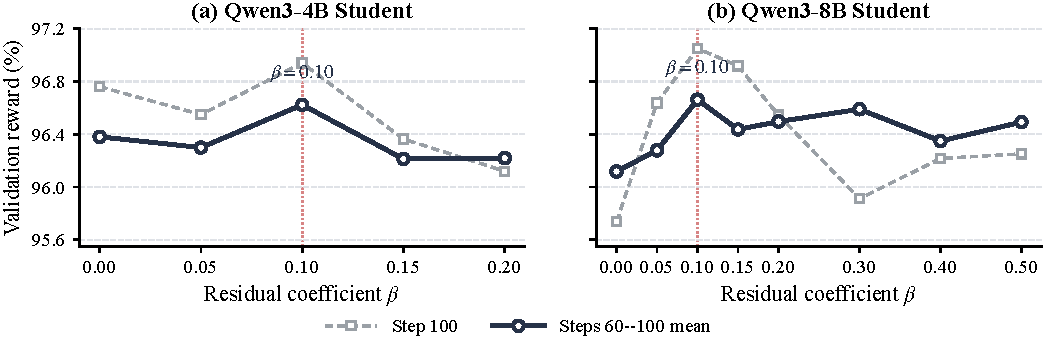
\includegraphics[width=\GCOPDValidationFigureWidth]{Figures/gcopd_validation/gcopd_beta_validation.pdf}
\caption{Held-out validation used to select the residual coefficient $\beta$. The fixed set contains 231 GoLongRL examples after 32K-token filtering and has no overlap with training. White squares show the step-100 reward. Circles show the mean over steps 60, 70, 80, 90, and 100. Both summaries select $\beta=0.10$ at both model scales.}
\label{fig:beta-validation}
\end{figure}

\ifdefined\GCOPDSingleColumnLayout
\ifdefined\GCOPDSingleColumnLayout
\begin{table}[t]
\else
\begin{table*}[t]
\fi
\caption{Qwen3-4B and Qwen3-8B results on five long-context benchmarks (\%). ``Avg.'' is the unweighted five-task mean. $\dagger$ denotes an implementation of the method's principal training-signal mechanism under the shared setup.}
\label{tab:main-results}
\centering
\small
\setlength{\tabcolsep}{4.0pt}
\begin{tabular}{l l c c c c c c }
\toprule
\multirow{2}{*}{\bf Model} & \multirow{2}{*}{\bf Method} & \multicolumn{6}{c}{\bf Benchmark} \\
\cmidrule(lr){3-8}
& & \bf Avg. & \bf DocMath & \bf Frames & \bf MRCR & \bf CorpusQA & \bf LBv1QA \\
\cmidrule(lr){1-2} \cmidrule(lr){3-8}
\multirow{7}{*}{Qwen3-4B}
& Raw & 29.08 & 43.63 & 26.58 & 22.02 & 6.99 & 46.20 \\
& OPD & 39.31 & 49.37 & \underline{30.95} & 26.90 & 32.22 & \textbf{57.10} \\
& ExOPD$^{\dagger}$ & 38.22 & 47.75 & 29.61 & 25.95 & 31.91 & 55.90 \\
& Uni-OPD$^{\dagger}$ & 38.53 & \textbf{51.88} & 29.98 & 27.93 & 27.36 & 55.50 \\
& PowerOPD$^{\dagger}$ & 38.88 & 49.63 & 30.10 & \textbf{28.36} & \underline{32.52} & 53.80 \\
& FiRe-OPD$^{\dagger}$ & \underline{39.50} & 49.37 & \textbf{31.31} & \underline{28.20} & \underline{32.52} & \underline{56.10} \\
\cmidrule(lr){2-2} \cmidrule(lr){3-8}
& \textbf{\method{} (ours)} & \textbf{40.47} & \underline{50.38} & 30.34 & 27.82 & \textbf{37.99} & 55.80 \\
\cmidrule(lr){1-2} \cmidrule(lr){3-8}
\multirow{7}{*}{Qwen3-8B}
& Raw & 35.12 & 45.88 & 30.95 & 23.87 & 22.19 & 52.70 \\
& OPD & 43.56 & \underline{55.13} & \textbf{34.59} & 30.44 & 39.82 & 57.80 \\
& PowerOPD$^{\dagger}$ & 41.53 & 51.38 & 32.65 & \underline{31.65} & 37.39 & 54.60 \\
& Uni-OPD$^{\dagger}$ & 43.41 & 54.13 & \textbf{34.59} & 25.25 & \underline{42.86} & \underline{60.20} \\
& ExOPD$^{\dagger}$ & 43.49 & 53.12 & 33.50 & \textbf{32.73} & 37.69 & \textbf{60.40} \\
& FiRe-OPD$^{\dagger}$ & \underline{44.01} & 54.00 & \underline{34.34} & 30.96 & 41.64 & 59.10 \\
\cmidrule(lr){2-2} \cmidrule(lr){3-8}
& \textbf{\method{} (ours)} & \textbf{44.65} & \textbf{55.50} & \textbf{34.59} & 31.10 & \textbf{43.77} & 58.30 \\
\bottomrule
\end{tabular}
\ifdefined\GCOPDSingleColumnLayout
\end{table}
\else
\end{table*}
\fi

\fi

\subsection{Main Results}

\paragraph{\method{} improves performance across model scales.}
As shown in Table~\ref{tab:main-results}, \method{} achieves the highest five-task average for both students. Relative to vanilla OPD, it raises the average score from 39.31 to 40.47 for Qwen3-4B and from 43.56 to 44.65 for Qwen3-8B. It also achieves the highest average among the evaluated shared-setup implementations at both model scales. Competing methods often lead on individual benchmarks but do not maintain the strongest aggregate performance. \method{} therefore provides a more favorable balance across the heterogeneous evaluation suite rather than relying on a single task.

\paragraph{Gains concentrate on structured reasoning and evidence aggregation.}
Relative to vanilla OPD, \method{} improves DocMath, MRCR, and CorpusQA for both students, with the largest gains on CorpusQA. These benchmarks emphasize structured reasoning and evidence aggregation. The concentration of gains is consistent with the intended role of response-level verifier calibration, although the table alone does not isolate task-specific mechanisms. Frames and LBv1QA show smaller or model-dependent changes, so the benefit is not uniform across tasks. Improvements over Raw confirm the effectiveness of the complete long-context post-training pipeline, whereas comparisons with vanilla OPD isolate the additional contribution of \method{}. The following ablations separately test the signed residual and its token-allocation rule.

\subsection{Ablation Studies}

We next examine the two components introduced by GC-OPD: the signed residual and RACA token allocation. All ablations use independently trained Qwen3-8B students under the shared setup and 100-step budget. We first vary the signal added to vanilla OPD while holding the coefficient and token-allocation rule fixed. We then examine how the residual should be distributed across tokens. Detailed formulations of all ablation variants are provided in Appendix~\ref{sec:ablation-configurations}.

\paragraph{Residualization improves upon OPD-only and direct-reward controls.}
Table~\ref{tab:residual-signal-ablation} isolates the signal added to vanilla OPD. The three augmented variants share RACA and $\beta=0.10$, so only the added term changes:
\begin{equation}
A'^{(i)}_t=A^{(i)}_t+
\begin{cases}
0, & \text{Vanilla OPD},\\
\beta c^{(i)}_t A^{(i)}_t, & \text{Additional OPD},\\
\beta c^{(i)}_t\tilde{R}^{(i)}, & \text{Direct reward},\\
\beta c^{(i)}_t\rho^{(i)}, & \text{GC-OPD}.
\end{cases}
\label{eq:signal-ablation-updates}
\end{equation}
Additional OPD changes the average score only from 43.56 to 43.60, indicating that another OPD-derived term does not explain the improvement. Direct reward reaches 44.19, confirming that group-normalized verifier feedback complements dense OPD guidance. Replacing the direct reward with the signed residual further raises the average score to 44.65 under the same coefficient and token-allocation rule. This additional gain supports accounting for the relative preference already expressed by OPD rather than adding verifier feedback alone.

\ifdefined\GCOPDSingleColumnLayout
\begin{table}[ht]
\else
\begin{table*}[ht]
\fi
\caption{Response-level signal ablation on Qwen3-8B. All augmented variants use RACA with coefficient $\beta=0.10$ and differ only in whether the added signal is $A^{(i)}_t$, $\tilde{R}^{(i)}$, or $\rho^{(i)}=\tilde{R}^{(i)}-\tilde{s}^{(i)}$. ``Avg.'' is the unweighted five-task mean, and ``$\Delta$'' is computed from the unrounded average relative to vanilla OPD.}
\label{tab:residual-signal-ablation}
\centering
\small
\setlength{\tabcolsep}{4.0pt}
\begin{tabular}{l c c c c c c c}
\toprule
\bf Variant & \bf Avg. & \bf DocMath & \bf Frames & \bf MRCR & \bf CorpusQA & \bf LBv1QA & $\boldsymbol{\Delta}$ \\
\cmidrule(lr){1-1} \cmidrule(lr){2-8}
Vanilla OPD & 43.56 & 55.13 & 34.59 & 30.44 & 39.82 & 57.80 & -- \\
Additional OPD & 43.60 & 54.63 & 34.59 & 30.03 & 39.51 & 59.20 & $+0.04$ \\
Direct reward & 44.19 & 55.13 & 34.59 & 30.40 & 40.73 & \textbf{60.10} & $+0.63$ \\
\cmidrule(lr){1-1} \cmidrule(lr){2-8}
\textbf{GC-OPD} & \textbf{44.65} & \textbf{55.50} & 34.59 & \textbf{31.10} & \textbf{43.77} & 58.30 & $\mathbf{+1.10}$ \\
\bottomrule
\end{tabular}
\ifdefined\GCOPDSingleColumnLayout
\end{table}
\else
\end{table*}
\fi


\paragraph{RACA improves residual allocation.}
Having established the contribution of the residual, we next examine its token allocation. Table~\ref{tab:token-credit-ablation} uses vanilla OPD as the no-residual anchor. All residual variants use $A'^{(i)}_t=A^{(i)}_t+0.10c^{(i)}_t\rho^{(i)}$ and differ only in $c^{(i)}_t$. Uniform sets $c^{(i)}_t=1$. Absolute OPD assigns credit using
\begin{equation}
c^{(i)}_t=\operatorname{clip}_{[0,5]}\!\left(
\frac{\lvert A^{(i)}_t\rvert}
{(T^{(i)})^{-1}\sum_{v=1}^{T^{(i)}}\lvert A^{(i)}_v\rvert}
\right),
\label{eq:absolute-opd-allocation}
\end{equation}
whereas RACA uses Equation~\ref{eq:raca}.

Uniform allocation raises the average score from 43.56 to 44.28, showing that the signed residual is useful even without token-dependent credit. RACA further raises it to 44.65, whereas Absolute OPD reaches only 43.93. Because Absolute OPD discards the sign of the OPD advantage, it can assign large credits to strongly negative OPD values. This result supports preserving the signed within-response ordering used by RACA.

\ifdefined\GCOPDSingleColumnLayout
\begin{table}[ht]
\else
\begin{table*}[ht]
\fi
\caption{Token-credit ablation on Qwen3-8B. All residual variants use the same signed residual with $\beta=0.10$ and differ only in token allocation. ``Avg.'' is the unweighted five-task mean, and ``$\Delta$'' is computed from the unrounded average relative to vanilla OPD.}
\label{tab:token-credit-ablation}
\centering
\small
\setlength{\tabcolsep}{4.0pt}
\begin{tabular}{l c c c c c c c}
\toprule
\bf Token allocation & \bf Avg. & \bf DocMath & \bf Frames & \bf MRCR & \bf CorpusQA & \bf LBv1QA & $\boldsymbol{\Delta}$ \\
\cmidrule(lr){1-1} \cmidrule(lr){2-8}
Vanilla OPD & 43.56 & 55.13 & 34.59 & 30.44 & 39.82 & 57.80 & -- \\
Absolute OPD & 43.93 & 54.63 & 35.56 & 29.53 & 41.34 & 58.60 & $+0.38$ \\
Uniform & 44.28 & 54.12 & \textbf{37.01} & 30.64 & 40.12 & \textbf{59.50} & $+0.72$ \\
\cmidrule(lr){1-1} \cmidrule(lr){2-8}
\textbf{RACA} & \textbf{44.65} & \textbf{55.50} & 34.59 & \textbf{31.10} & \textbf{43.77} & 58.30 & $\mathbf{+1.10}$ \\
\bottomrule
\end{tabular}
\ifdefined\GCOPDSingleColumnLayout
\end{table}
\else
\end{table*}
\fi


\ifdefined\GCOPDSingleColumnLayout
\FloatBarrier
\fi

\subsection{Disagreement Across Task Families}

Beyond downstream performance, we use a fixed response set to test whether teacher--verifier disagreement extends beyond the two tasks in Figure~\ref{fig:teacher-verifier-motivation}. This diagnostic measures disagreement prevalence rather than trained-checkpoint performance.

\paragraph{Teacher--verifier disagreement extends across task families.}
Figure~\ref{fig:task-conditioned-mismatch} in Appendix~\ref{sec:task-conditioned-disagreement} reports pairwise disagreement and top-1 mismatch for four task families containing at least 500 prompts, together with a prompt-macro aggregate over all nine families. The Multi-Table Extraction and High-Recall Retrieval rows aggregate the same frozen responses used in Figure~\ref{fig:teacher-verifier-motivation} over prompts shorter than 32K. The additional task rows show that disagreement extends beyond these two tasks, while the variation across rows indicates that its prevalence remains task dependent.
